% $HeadURL$
\subsection{Glyph: \glyph{Macromolecule}}
\label{sec:macromolecule}

Many biological processes involve \emph{macromolecules}: biochemical substances that are built up from the covalent linking of pseudo-identical units.
Examples of macromolecules include proteins, nucleic acids (RNA, DNA), and polysaccharides (glycogen, cellulose, starch, etc.).
Attempting to define a separate glyph for all of these different molecules would lead to an explosion of symbols in SBGN, so instead, \SBGNPDLone specifies only one glyph for all macromolecules.
The same glyph is to be used for a protein, a nucleic acid, a complex sugar, and so on.
The exact nature of a particular macromolecule in a map is then clarified using its label and decorations, as it will become clearer below.
% 
(Future levels of SBGN may subclass the \glyph{macromolecule} and introduce different glyphs to differentiate between types of macromolecules.)

\begin{glyphDescription}

\glyphSboTerm
SBO:0000245 ! macromolecule


\glyphIncoming
Zero or more \glyph{production} arcs (\sect{production}).



\glyphOutgoing
Zero or more \glyph{consumption} arcs (\sect{consumption}), \glyph{modulation arcs} (\sect{modulations}), \glyph{logic arcs} (\sect{logicArc}), or \glyph{equivalence arcs} (\sect{equivalenceArc}).


\glyphContainer
A \glyph{macromolecule} is represented by a rectangular shape with rounded corners, as shown in \fig{macromolecule}.

\glyphLabel
A \glyph{macromolecule} is identified by a label  that is a string of characters that may be distributed on several lines to improve readability.
The centre of the label must be placed on the centre of the container.
The label may extend outside of the container.

\glyphAux
A \glyph{macromolecule} can carry one or more \glyph{state variables} that add information about its state (\sect{stateVariable}).
The state of a \glyph{macromolecule} is defined as the set of all its \glyph{state variables}.

A \glyph{macromolecule} can also carry one or more \glyph{units of information} (\sect{unitInfo}).
These can characterise a domain, such as a binding site.
Particular \glyph{units of information} are available for describing the material type (\sect{material-types-cv}) and the conceptual type (\sect{conceptual-types-cv}) of a \glyph{macromolecule}.

Finally, a \glyph{macromolecule} can also carry a \glyph{labelled clone marker} (see \sect{cloneMarker}).

\end{glyphDescription}

\begin{figure}[H]
  \centering
  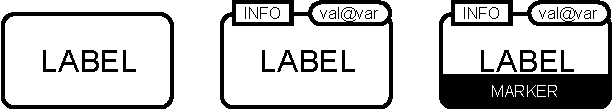
\includegraphics{images/macromolecule-combined}% \hspace*{2em}
  %\raisebox{0.04in}{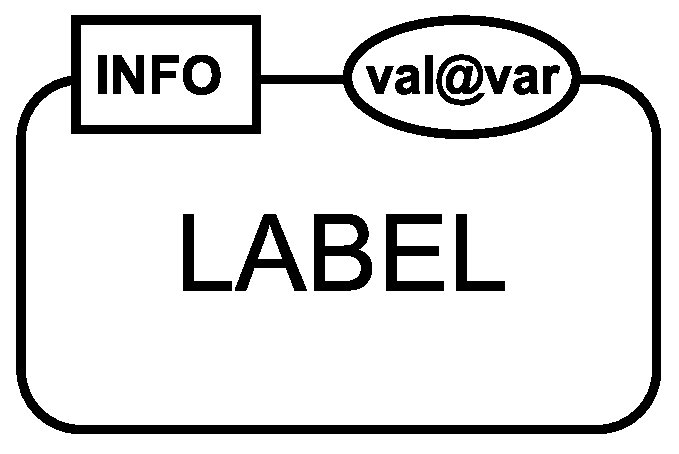
\includegraphics[width = 1.25in]{images/macromolecule}}
  \caption{The \PD glyph for \glyph{macromolecule}, shown plain and unadorned on the left, with an additional \glyph{state variable} and a \glyph{unit of information} in the middle, and with a \glyph{labelled clone marker} on the right.}
  \label{fig:macromolecule}
\end{figure}

% The following is for [X]Emacs users.   Please leave in place.
% Local Variables:
% TeX-master: "../sbgn_PD-level1"
% End:
